 \chapter{Case Studies}

This chapter presents the implementation of several applications in MELON. The code examples are written using the Ruby implementation of MELON in order to demonstrate concrete usage of MELON operations.

\section{News Server/Reader}

In this section, we consider news servers which produce news reports, each with a category and a headline. News readers use a client which fetches all news headlines from a given category.

\begin{lstlisting}[caption={News Server}, label={code:newsserver}]
class NewsServer
  def initialize
    @melon = Melon.new
  end

  def report(category, headline)
    @melon.write([category, headline])
  end
end
\end{lstlisting}



A class implementing the news server is shown in Listing \ref{code:newsserver}. To ensure all interested parties can read the news, the server uses \textbf{write} to disallow a reader from removing a news item and preventing other readers from reading it. When a news item is reported, the server simply writes a message containing the category and headline.

Multiple news servers may be producing news reports at the same time.

\begin{lstlisting}[caption={News Reader}, label={code:newsreader}]
class NewsReader
  def initialize
    @melon = Melon.new
  end

  def fetch(category)
    @melon.read_all([category, String])
  end
end
\end{lstlisting}

The news reader is just as simple, as shown in Figure \ref{code:newsreader}. The \texttt{fetch} method will fetch all reports in the given category. Repeated calls to \texttt{fetch} will only return news reports which have not already been read. The method will block if no new reports are available.

\section{Chat Application}

Basic chat applications are a common example of networked communications. Participants broadcast messages tagged with their name, which are received by all participants.

\begin{lstlisting}[caption={Chat Application}, label={code:chat}]
class Chat
  def initialize name
    @name = name
    @melon = Melon.new
  end

  def chat(message)
    @melon.write([@name, message])
  end

  def read_messages
    @melon.read_all([String, String])
  end

  def start
    monitor
    loop do
      print "? "
      message = gets.strip
      chat message unless message.empty?
    end
  end

  def monitor
    Thread.new do
      loop { print_messages(read_messages) }
    end
  end
  
  def print_messages(messages)
    messages.each do |name, message|
      puts "\n<#{name}> #{message}" unless name == @name
    end
  end
end
\end{lstlisting}

The class in Listing \ref{code:chat} implements a simple command-line chat client. When the \texttt{start} method is called, the client starts a new thread which reads and shows any messages sent by other chatters. Note the \texttt{print\_messages} method filters out messages sent by the current chatter (this assumes everyone has a unique name). This is because the \texttt{read\_messages} method will pull in all unread messages, even those sent by the current client. A more sophisticated message matching system would be able to provide negative template values (i.e., "match any string which does not match this pattern"), but for our prototype this is not possible.

In the main thread, the client requests messages from the current chatter and sends them using the \texttt{chat} method. The \texttt{chat} method then simply wraps the message in an array with the chatter's name as the first value, then sends the message using \textbf{write}, since we want the message to be available for many chatters to read.

As usual, messages from a single chatter will always be received in the order the messages were sent, but no order is imposed across all chatters.

\section{Job Queue}

In a job queue, tasks are added to a shared queue. Workers remove tasks from the queue and execute them. Naturally, access to the queue should be atomic to maintain consistency and a job should only be executed by a single worker.

\begin{lstlisting}[caption={Job Producer}, label={code:jobproducer}]
class Producer
  def initialize
    @melon = Melon.new
  end

  def add_job(job)
    @melon.store([job])
  end
end
\end{lstlisting}

The job producer in Listing \ref{code:jobproducer} does very little, just saves the jobs in the MELON shared storage using \textbf{store}. Jobs are assumed to be a subclass of a \texttt{Job} class with an \texttt{execute} method to be called by the workers. Any number of producers may add jobs to the queue.

\begin{lstlisting}[caption={Worker}, label={code:worker}]
class Worker 
  def initialize
    @melon = Melon.new
  end

  def fetch_job
    @melon.take([Job])[0]
  end

  def work
    loop do
      fetch_job.execute
    end
  end
end
\end{lstlisting}

Workers retrieve jobs using \textbf{take} and invoke the \texttt{execute} method on them. If no jobs are available, the worker will block. Since MELON's \textbf{take} operation is atomic, there is no danger of a job being run by more than a single worker. If there is only a single job producer, the jobs will be executed in first-in, first-out order as enforced by MELON semantics.

\section{Experiment Coordinator}

\begin{figure}
\centering
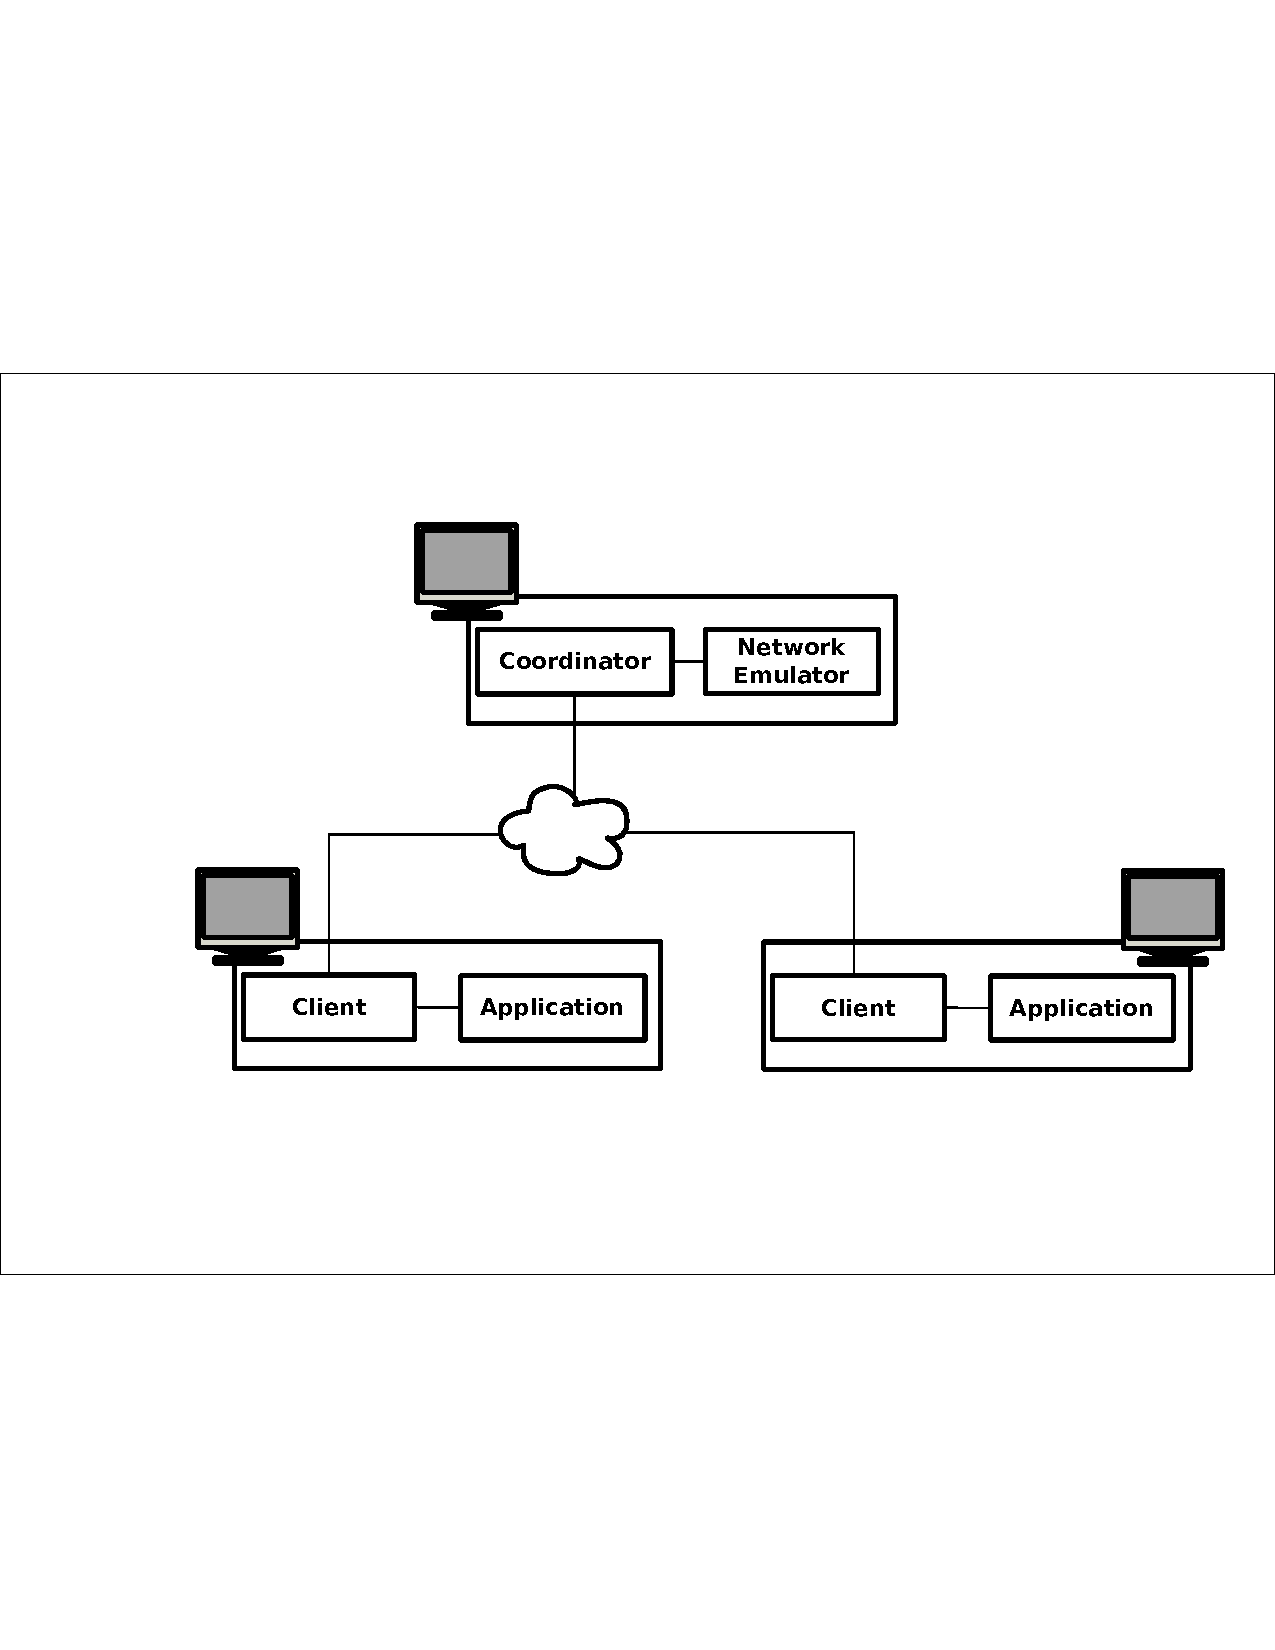
\includegraphics[scale = .75, clip, trim = 94px 279px 24px 252px]{figures/experiment_arch.pdf}
\caption{Coordinator Architecture}
\label{fig:coordarchitecture}
\end{figure}

This case study examines an application developed and used to generate the experimental results in Chapter \ref{chapter:evaluation}. To ease the process of repeatedly setting up experiments, we developed an experiment coordination framework written with MELON. The framework handles running real applications on multiple hosts, executing the network emulator, and gathering results into a single location.

The architecture of the framework is illustrated in Figure \ref{fig:coordarchitecture}. For simplicity, the coordinator resides on the same host as the network emulator. The coordinator sends out commands to clients which reside on each host. The clients are responsible for executing programs on their local host and sending resulting output back to the central coordinator.

When running the coordinator, the number of clients and their IP addresses is known. This simplifies operations but also allows an experiment to be run with a specific number of nodes. It is also possible to set two different commands to be run on different types of nodes. For example, one node can be a ``source" and run one command, while the other nodes are ``sinks" and run a separate command.

\begin{table}\footnotesize
\centering
\caption{Coordination Framework Messages}
\begin{tabular}{|c|c|c|}
\hline
Coordinator & Clients & Description \\ \hline
 & \textbf{read}([type, String]) & Await command \\ \hline
\textbf{write}([``client", client\_command]) & & Send client command \\ \hline
\textbf{write}([``server", server\_commnad]) & & Send server command \\ \hline
\textbf{take}([``confirm", ip]) & & Wait confirmations \\ \hline
 & \textbf{store}([``confirm", ip]) & Store confirmation \\ \hline
 & \textbf{read}([``go"]) & Await go signal \\ \hline
\textbf{write}([``go"]) & & Send go signal \\ \hline
\textbf{take}([``done", ip]) & & Wait for clients to finish \\ \hline
& \textbf{store}([``result", ip, output]) & Store results \\ \hline
& \textbf{store}([``done", ip]) & Store done signal \\ \hline
& \textbf{read}([``finished"]) & Await finished signal \\ \hline
\textbf{take\_all}([``result", String, String]) & & Gather results \\ \hline
\textbf{write}([``finished"]) & & Send finished signal \\ \hline
\end{tabular}
\label{table:framework}
\end{table}

Table \ref{table:framework} lists an overview of the MELON commands used to communicate between the coordinator process and the client processes. The order of communications are not always strict. For example, it does not matter if the coordinator first sends the commands and then the clients wait, or if the clients wait first. In practice, these operations will be concurrent. Coordination between processes is achieved by blocking on messages containing signals (``confirm'', ``go'', ``done'', etc.)

When starting, the coordinator writes a message for each command type (called ``server" and ``client" for convenience). Then it performs a \textbf{take} operation for a confirmation message from each client IP address. Each client reads the relevant command, starts the command, waits for the application to initialize, then uses \textbf{store} to send a confirmation message with its IP address.

When the coordinator has taken a confirmation from each host, it starts the network emulator, then writes a ``go'' message. Upon reading the ``go" message, each client signals the application to begin. The coordinator then blocks waiting on ``done" messages from each client.

As the application runs, the client reads the output line by line and stores each line using \textbf{store}, labeled with the client's IP address. When the application finishes, the client stores a ``done'' signal. When the coordinator has taken a ``done'' message from each client, it collects the results and then sends a ``stop'' message. The clients then stop the applications and the framework is ready to start the next experiment.

Unlike the other examples in this chapter, this application was developed to fill an actual need, as opposed to being strictly a demonstration of how to use MELON. We have used all of MELON's operations except \textbf{read\_all} in this application. Read-only operations were used to broadcast messages from the coordinator to the clients, while \textbf{store}/\textbf{take} operations were used to send messages back to the coordinator. The default blocking behavior for \textbf{read}/\textbf{take} were useful to coordinate actions.

In our usage of the experiment coordination framework, the output from the applications were stored and organized by the coordinator into separate files by client. Since MELON retrieves messages in order per host, no ordering information needs to be included in the output messages. The coordinator merely writes the messages out to the proper file (by client IP address, which is included in the message) in the order it received them.

\section{Shared Whiteboard}\label{sec:wb}

This section presents the implementation of a shared whiteboard not only using MELON, but also publish/subscribe, RPC, and tuple spaces in order to compare their features and performance.

A shared whiteboard is a digital document which may be edited and viewed by multiple users concurrently and is commonly proposed as an example of an application well-suited to MANETs\cite{wb5}\cite{wb6}. Shared whiteboards are distributed, real-time, and interactive, which presents some interesting characteristics. Since many participants may be updating the whiteboard, ordering of changes is very important to maintain a consistent document. It is also important that changes be propagated quickly so that each user is working with the latest document.

Each version shares common code related to the actual whiteboard itself, which is implemented in the \texttt{Whiteboard} class. Changes to the shared whiteboard are encapsulated in a \texttt{Figure} object. Each version implements an \texttt{add\_local\_figure} method which is called when the user modifies the shared whiteboard. The MELON and tuple space versions also implement an \texttt{add\_remote\_figures} method which is used to retrieve updates from remote nodes.

\subsection{Publish/Subscribe}

The publish/subscribe paradigm divides processes into publishers and subscribers. In topic-based publish/subscribe, publishers simply publish messages tagged with a topic identifier. Subscribers receive the messages by subscribing to one or more topics and specifying a callback to handle the publications asynchronously and separately from the main process thread. It is also possible to handle multiple incoming publications concurrently. Publish/subscribe does not guarantee any ordering of publications nor does it specify how to deliver messages if the subscribers is not available at the time of publication. In distributed publish/subscribe such as MANETs, it is generally not expected that publishers would persist and deliver messages at a later time\cite{psfaces}.

The publish/subscribe whiteboard in Table \ref{fig:pswb} sets up a subscription to the ``whiteboard" topic and a callback to add remotely published figures to the whiteboard. This allows the whiteboard to receive updates at any time in a separate thread, which is precisely what would be desired. To output a new figure, the whiteboard simply publishes the figure to the ``whiteboard" topic.

\begin{table}
\centering
\begin{tabular}{c c}
\begin{minipage}{2.75in}
\begin{verbatim}
require "ps"
require "whiteboard"

class PSWhiteboard < Whiteboard
  def initialize
    @ps = PS.new
    
    @ps.subscribe("whiteboard") do |figure|
      add_figure(figure)
    end
  end

  def add_local_figure(figure)
    @ps.publish("whiteboard", figure)
  end
end
\end{verbatim}
\caption{Publish/Subscribe Whiteboard}\label{fig:pswb}
\end{minipage}
&
\begin{minipage}{2.5in}
\begin{verbatim}
require "rpc"
require "whiteboard"

class RPCWhiteboard < Whiteboard
  def initialize
    @rpc = RPC.new
    @rpc.export(self)
  end

  def add_local_figure(figure)
    wbs = @rpc.find_all("RPCWhiteboard")
    wbs.add_figure(figure)
  end
end


\end{verbatim}
\caption{RPC Whiteboard}\label{fig:rpcwb}
\end{minipage}
\end{tabular}
\end{table}


\subsection{RPC}

Remote procedure calls (RPC) is a distributed programming paradigm which disguises remote communication as local method calls. A host can ``export" an object to be accessed remotely. Remote hosts discover these remote objects by name and then invoke methods on them. Arguments may be passed to the remote method and the return value of the method is returned to the local process. A variation of this used in our example is group RPC, which allows us to invoke the same method with the same arguments on all known remote objects of the requested type. These calls are performed asynchronously. Typically the return values would be handled by a callback, but this functionality is not used in our example.

A shared whiteboard implementation using RPC is listed in Table 5. When the whiteboard is initialized, it exports itself as a remote object. This allows other hosts to remotely invoke the \texttt{add\_figure}. Like publish/subscribe, this allows the whiteboard to accept remote figures asynchronously from the main process thread and is a natural feature of RPC. Distribution of remote figures is performed by first finding all remote instances of \texttt{RPCWhiteboard}, then invoking the \texttt{add\_figure} method (defined on the parent class) directly, passing in the new figure as an argument. Since the group RPC is asynchronous, it is possible that a call might complete before a prior call.

\subsection{Tuple Spaces}

Tuple spaces operate on a distributed shared memory space of ordered tuples. Tuples may be output using the \textbf{out} operation, then retrieved using \textbf{rd}, which copies the tuple, or \textbf{in}, which removes the tuple from the tuple space based on matching templates. If multiple tuples match a template, one of the matching tuples is chosen nondeterministically to be returned.

Table \ref{fig:tswb} shows the tuple space version, which is very similar to MELON. To send an update, it outputs a tuple containing just the new figure. Unlike MELON, a misbehaving or misconfigured client could remove the messages from the tuple space, disrupting the shared whiteboard communication. Retrieval of remote messages uses a \textbf{bulk\_rd} operation to read all messages containing a figure. To continuously retrieve messages asynchronously, this method can be called inside a loop in a separate thread. Once a group of figures is retrieved, each individual figure is added to the local whiteboard.

Tuple spaces suffer from the multiple read problem\cite{mrdp}: repeated nondestructive read operations (\textbf{rd}) may return any matching tuple, including the same tuple. As discussed in \cite{mrdp}, one solution is to use a mutex tuple to gain exclusive access to the tuple space, remove all the desired tuples using \textbf{in}, then replace all the tuples and release the mutex. However, this approach prevents concurrent access and is dangerous in a MANET where the node holding the mutex may disappear. Another solution is to use a counter in each tuple, then read tuple 0, then tuple 1, and so on. Then each process can request tuples by the counter value. However, if multiple processes are producing tuples they must coordinate to produce consistent counters, essentially resulting in a producer-side mutex.

Finally, \cite{mrdp} proposes a \textbf{copy-collect} operation, which copies all matching tuples. We have implemented this as the \textbf{bulk\_rd} operation as used in Table \ref{fig:tswb}. However, this does not solve what might be termed the ``multiple multiple read problem": since our tuple space is not static, reading all matching tuples once is not sufficient. We need to be able to perform multiple \textbf{bulk\_rd}s to get all figures added to the whiteboard. Without \textit{a prior} knowledge of remote hosts in the system, the only option which allows concurrent access to the tuple space is to read \textit{all} matching tuples. Naturally, this becomes quite expensive as the number of tuples grows.

\begin{table}
\centering
\begin{tabular}{c c}
\begin{minipage}{2.75in}
\begin{verbatim}
require "melon"
require "whiteboard"

class MelonWhiteboard < Whiteboard
  def initialize
    @melon = Melon.new
  end
  
  def add_local_figure(figure)
    @melon.write([Figure])
  end

  def add_remote_figures
    figures = @melon.read_all([Figure])

    figures.each do |figure|
      add_figure(figure[0])
    end
  end
end
\end{verbatim}
\caption{MELON Whiteboard}\label{fig:mwb}
\end{minipage}
&
\begin{minipage}{2.5in}
\begin{verbatim}
require "tuplespace"
require "whiteboard"

class TSWhiteboard < Whiteboard
  def initialize
    @ts = Tuplespace.new
  end

  def add_local_figure(figure)
    @ts.out([Figure])
  end

  def add_remote_figures
    figures = @ts.bulk_rd([Figure])

    figures.each do |figure|
      add_figure(figure[0])
    end
  end
end 
\end{verbatim}
\caption{Tuple Space Whiteboard}\label{fig:tswb}
\end{minipage}
\end{tabular}
\end{table}

\subsection{MELON}

The MELON whiteboard in Table \ref{fig:mwb} writes out each figure in a tuple containing just the new figure. It uses the \textbf{write} operation since every remote node needs to be able to read the figures. To retrieve remote figures, MELON uses \textbf{read\_all} to nondestructively read all messages containing a \texttt{Figure}. Like tuple spaces, the \texttt{add\_remote\_figures} method should be called in a separate thread to provide asynchronous updates. Unlike tuple spaces, MELON's \textbf{read\_all} operation only retrieves unread messages, eliminating the ``multiple multiple read" problem.

MELON directly provides three features which are helpful to the whiteboard application: persistent messages, reading only unread messages, and returning messages in a per-host ordering. Message persistence is crucial in MANET applications, where communication with remote nodes is often disrupted and delayed. For a shared whiteboard, every message must be delivered to keep the document synchronized between users. By managing read versus unread messages, MELON easily allows the whiteboard to efficiently fetch only newly-added figures. Finally, MELON guarantees the updates from each host will be retrieved in the order that host initiated them. While this does not provide a global ordering, it does ensure updates from a single host will be in order.

\section{Summary}

MELON provides simple, yet powerful operations for communicating and coordinating between hosts and processes.

In none of the code examples using MELON was it necessary 